\documentclass[10pt]{article}
\usepackage{tikz}
\usetikzlibrary{shapes.misc}
\usepackage[margin=0cm]{geometry}
\pagestyle{empty}
\tikzstyle{every node}=[cross out, draw, red]

\begin{document}

\vspace*{\fill}
\begin{center}
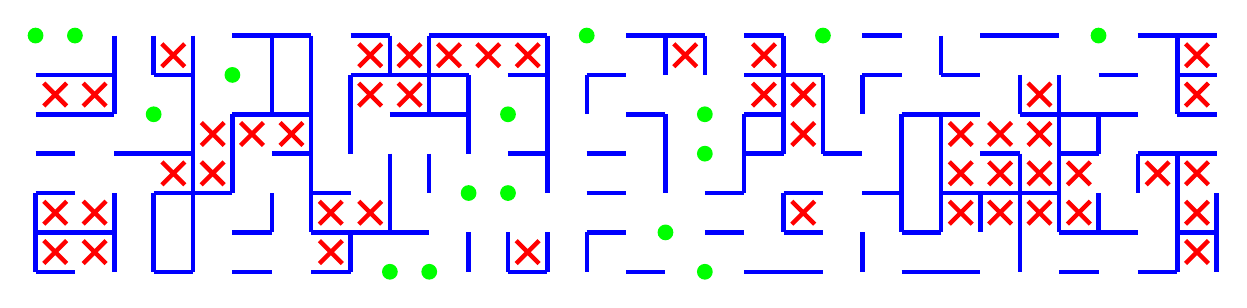
\begin{tikzpicture}[x=0.5cm, y=-0.5cm, ultra thick, blue]
% Walls
    \draw (5,0) -- (7,0);
    \draw (8,0) -- (9,0);
    \draw (10,0) -- (13,0);
    \draw (15,0) -- (17,0);
    \draw (18,0) -- (19,0);
    \draw (21,0) -- (22,0);
    \draw (24,0) -- (26,0);
    \draw (28,0) -- (30,0);
    \draw (0,1) -- (2,1);
    \draw (3,1) -- (4,1);
    \draw (8,1) -- (11,1);
    \draw (12,1) -- (13,1);
    \draw (14,1) -- (15,1);
    \draw (18,1) -- (20,1);
    \draw (21,1) -- (22,1);
    \draw (23,1) -- (24,1);
    \draw (27,1) -- (28,1);
    \draw (29,1) -- (30,1);
    \draw (0,2) -- (2,2);
    \draw (5,2) -- (7,2);
    \draw (9,2) -- (11,2);
    \draw (15,2) -- (16,2);
    \draw (18,2) -- (19,2);
    \draw (22,2) -- (24,2);
    \draw (25,2) -- (28,2);
    \draw (29,2) -- (30,2);
    \draw (0,3) -- (1,3);
    \draw (2,3) -- (4,3);
    \draw (6,3) -- (7,3);
    \draw (12,3) -- (13,3);
    \draw (14,3) -- (15,3);
    \draw (18,3) -- (19,3);
    \draw (20,3) -- (21,3);
    \draw (24,3) -- (25,3);
    \draw (26,3) -- (27,3);
    \draw (28,3) -- (30,3);
    \draw (0,4) -- (1,4);
    \draw (3,4) -- (5,4);
    \draw (7,4) -- (8,4);
    \draw (14,4) -- (15,4);
    \draw (17,4) -- (18,4);
    \draw (19,4) -- (20,4);
    \draw (21,4) -- (22,4);
    \draw (23,4) -- (26,4);
    \draw (0,5) -- (2,5);
    \draw (5,5) -- (6,5);
    \draw (7,5) -- (10,5);
    \draw (14,5) -- (15,5);
    \draw (17,5) -- (18,5);
    \draw (19,5) -- (20,5);
    \draw (22,5) -- (23,5);
    \draw (26,5) -- (28,5);
    \draw (29,5) -- (30,5);
    \draw (0,6) -- (1,6);
    \draw (3,6) -- (4,6);
    \draw (5,6) -- (6,6);
    \draw (7,6) -- (8,6);
    \draw (12,6) -- (13,6);
    \draw (15,6) -- (16,6);
    \draw (18,6) -- (20,6);
    \draw (22,6) -- (24,6);
    \draw (26,6) -- (27,6);
    \draw (28,6) -- (29,6);
    \draw (0,4) -- (0,6);
    \draw (2,0) -- (2,2);
    \draw (2,4) -- (2,6);
    \draw (3,0) -- (3,1);
    \draw (3,4) -- (3,6);
    \draw (4,0) -- (4,6);
    \draw (5,2) -- (5,4);
    \draw (6,0) -- (6,2);
    \draw (6,4) -- (6,5);
    \draw (7,0) -- (7,5);
    \draw (8,1) -- (8,3);
    \draw (8,5) -- (8,6);
    \draw (9,0) -- (9,1);
    \draw (9,3) -- (9,5);
    \draw (10,0) -- (10,2);
    \draw (10,3) -- (10,4);
    \draw (11,1) -- (11,3);
    \draw (11,5) -- (11,6);
    \draw (12,5) -- (12,6);
    \draw (13,0) -- (13,4);
    \draw (13,5) -- (13,6);
    \draw (14,1) -- (14,2);
    \draw (14,5) -- (14,6);
    \draw (16,0) -- (16,1);
    \draw (16,2) -- (16,4);
    \draw (17,0) -- (17,1);
    \draw (18,2) -- (18,4);
    \draw (19,0) -- (19,3);
    \draw (19,4) -- (19,5);
    \draw (20,1) -- (20,3);
    \draw (21,1) -- (21,2);
    \draw (21,5) -- (21,6);
    \draw (22,2) -- (22,5);
    \draw (23,0) -- (23,1);
    \draw (23,2) -- (23,5);
    \draw (24,4) -- (24,5);
    \draw (25,1) -- (25,2);
    \draw (25,3) -- (25,6);
    \draw (26,1) -- (26,5);
    \draw (27,2) -- (27,3);
    \draw (27,4) -- (27,5);
    \draw (28,3) -- (28,4);
    \draw (29,0) -- (29,2);
    \draw (29,3) -- (29,6);
    \draw (30,4) -- (30,6);
% Pillars
    \fill[green] (0,0) circle(0.2);
    \fill[green] (1,0) circle(0.2);
    \fill[green] (14,0) circle(0.2);
    \fill[green] (20,0) circle(0.2);
    \fill[green] (27,0) circle(0.2);
    \fill[green] (5,1) circle(0.2);
    \fill[green] (3,2) circle(0.2);
    \fill[green] (12,2) circle(0.2);
    \fill[green] (17,2) circle(0.2);
    \fill[green] (17,3) circle(0.2);
    \fill[green] (11,4) circle(0.2);
    \fill[green] (12,4) circle(0.2);
    \fill[green] (16,5) circle(0.2);
    \fill[green] (9,6) circle(0.2);
    \fill[green] (10,6) circle(0.2);
    \fill[green] (17,6) circle(0.2);
% Inner points in accessible cul-de-sacs
    \node at (3.5,0.5) {};
    \node at (8.5,0.5) {};
    \node at (9.5,0.5) {};
    \node at (10.5,0.5) {};
    \node at (11.5,0.5) {};
    \node at (12.5,0.5) {};
    \node at (16.5,0.5) {};
    \node at (18.5,0.5) {};
    \node at (29.5,0.5) {};
    \node at (0.5,1.5) {};
    \node at (1.5,1.5) {};
    \node at (8.5,1.5) {};
    \node at (9.5,1.5) {};
    \node at (18.5,1.5) {};
    \node at (19.5,1.5) {};
    \node at (25.5,1.5) {};
    \node at (29.5,1.5) {};
    \node at (4.5,2.5) {};
    \node at (5.5,2.5) {};
    \node at (6.5,2.5) {};
    \node at (19.5,2.5) {};
    \node at (23.5,2.5) {};
    \node at (24.5,2.5) {};
    \node at (25.5,2.5) {};
    \node at (3.5,3.5) {};
    \node at (4.5,3.5) {};
    \node at (23.5,3.5) {};
    \node at (24.5,3.5) {};
    \node at (25.5,3.5) {};
    \node at (26.5,3.5) {};
    \node at (28.5,3.5) {};
    \node at (29.5,3.5) {};
    \node at (0.5,4.5) {};
    \node at (1.5,4.5) {};
    \node at (7.5,4.5) {};
    \node at (8.5,4.5) {};
    \node at (19.5,4.5) {};
    \node at (23.5,4.5) {};
    \node at (24.5,4.5) {};
    \node at (25.5,4.5) {};
    \node at (26.5,4.5) {};
    \node at (29.5,4.5) {};
    \node at (0.5,5.5) {};
    \node at (1.5,5.5) {};
    \node at (7.5,5.5) {};
    \node at (12.5,5.5) {};
    \node at (29.5,5.5) {};
% Entry-exit paths without intersections
\end{tikzpicture}
\end{center}
\vspace*{\fill}

\end{document}
